\documentclass{beamer}

\setlength{\parskip}{\baselineskip}
\setlength{\parindent}{0pt}
\usepackage{default}
\usepackage{tabularx}
\usepackage{url}
\usepackage{graphicx}

\title{\huge{Using \texttt{git} for version control}}
\author{Manuel Baumann, Joost van Zwieten}
\titlegraphic{
   
\includegraphics[scale=0.08]{images/TU_Delft_logo1.png}\hspace{4cm}
\includegraphics[scale=0.15]{../../images/logo}}
\date{\footnotesize{November 28, 2013}}
\begin{document}

\frame{\titlepage}
\begin{frame}
\frametitle{What is Project baNaNa ?}
Many (math) presentations are far too technical and only some people in the audience can follow.

The aim of project ba\color{red}NaN\color{black}a is:
\begin{itemize}
 \item present every-day tools to each other,
 \pause
 \item informal/interactive presentations,
 \pause
 \item focus on software, applications, ...
 \pause
 \item a series of lectures for and by fellow PhD students,
 \pause
 \item there is no grading whatsoever, 
 \pause
 \item eating bananas together.
\end{itemize}
\end{frame}

\begin{frame}
\frametitle{What is Project baNaNa ?}
\framesubtitle{More details...}
In more detail, we were thinking about
\begin{itemize}
 \item possible topics:
 \begin{itemize}
 \item Python
 \item CUDA/OpenCL
 \item Open Foam
 \item MPI/OpenMP
 \item latex `best practice'
 \item high end Matlab usage
 \end{itemize}
 \item a classical lecture:
  \begin{itemize}
 \item approx. 20 mins
 \item once a month
 \item everybody contributes from time to time
 \item \textbf{gives many examples}
 \end{itemize}
\end{itemize}
\end{frame}
\begin{frame}
\frametitle{Today's lecture: \texttt{git}}
Do you know this situation?
\begin{figure}
\centering
 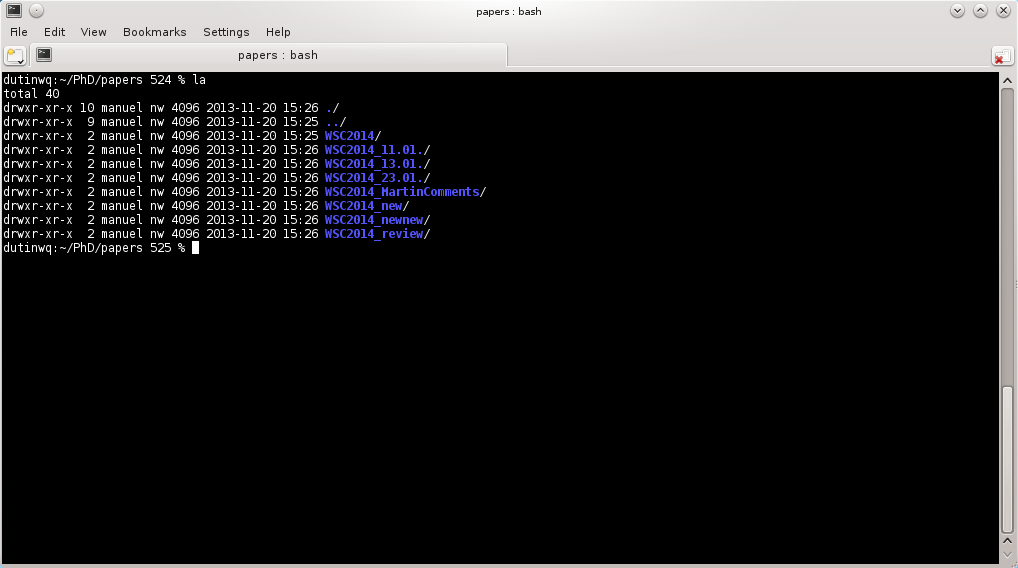
\includegraphics[height=0.64\textheight]{images/screenshot.png}
\end{figure}
\end{frame}

\begin{frame}
\frametitle{Today's lecture: \texttt{git}}
The pre-installed software package \texttt{git} can be used for version control for a (bigger) software project.
\begin{itemize}
 \item helps to keep track of changes in your project directory
 \item branching, merging
 \item collaboration
 \item several sites allow you to publish your \texttt{git} repository (github, bitbucket, gitorious) 
\end{itemize}
\end{frame}
\begin{frame}
\frametitle{Today's lecture: \texttt{git}}
\framesubtitle{More details...}
The most important commands:

\begin{table}
\begin{tabularx}{\textwidth}{l|X}
Command & Meaning \\
 \hline
 \texttt{git init} & First command, makes current folder a \texttt{git} repository\\
 \texttt{git add <file>} & Stages a file\\
 \texttt{git commit -m <message>} & Record changes to the repository\\
 \texttt{git status} & Show the working tree status\\
 \texttt{git diff} & Show changes between commits, commit and working tree, etc\\
\end{tabularx}
\end{table}
\hfill $\hookrightarrow$ live demonstration...
\end{frame}
\begin{frame}
\frametitle{Branching}
\framesubtitle{The typical work flow}
\end{frame}
\begin{frame}
\frametitle{Today's lecture: \texttt{git}}
\framesubtitle{More details...}
Even more important commands:
\begin{table}
\begin{tabularx}{\textwidth}{l|X}
Command & Meaning \\
 \hline
 \texttt{git branch} & List, create, or delete branches\\
 \texttt{git checkout} & Checkout a branch or paths to the working tree\\
 \texttt{git merge} & Join two or more development histories together\\
 \texttt{git mergetool} & Run merge conflict resolution tools to resolve merge conflicts\\
\end{tabularx}
\end{table}
\hfill $\hookrightarrow$ live demonstration...
\end{frame}
\begin{frame}
\frametitle{(Biased) Comparison \texttt{git} vs. \texttt{Dropbox}}
\begin{itemize}
 \item sensitive information should not be stored in Dropbox
 \item \texttt{git} branches are non-linear in time
 \item local argument: \texttt{git} is supported (and pre-installed) at TU Delft work stations
\end{itemize}
\end{frame}
\begin{frame}
\frametitle{Further reading}
Many information are available online:
\begin{itemize}
 \item \url{https://github.com/}
 \item \url{http://try.github.io/levels/1/challenges/1}
 \item \url{http://git-scm.com/book}
\end{itemize}
These slides, and much more, will be published at:
\begin{itemize}
 \item \url{http://projectbanana.github.io/}
\end{itemize}
 \begin{figure}
\centering
 
\includegraphics[height=0.3\textheight]{../../images/logo}
\end{figure}

\end{frame}
\end{document}
